\subsection{Unraveling the Magic of Method of Moments!}

\begin{tcolorbox}[colback=gray!10, colframe=black, title=E9B10] What is the principle of a Method of Moments analysis?
\begin{enumerate}[label=\Alph*.]
    \item \textbf{A wire is modeled as a series of segments, each having a uniform value of current}
    \item A wire is modeled as a single sine-wave current generator
    \item A wire is modeled as a single sine-wave voltage source
    \item A wire is modeled as a series of segments, each having a distinct value of voltage across it
\end{enumerate} \end{tcolorbox}

\subsubsection{Related Concepts}

The Method of Moments (MoM) is a numerical technique used primarily for analyzing electromagnetic problems, particularly those involving wire antennas and scatterers. This method is pivotal in computational electromagnetics and is predicated upon the principle of transforming a differential equation into a system of linear equations.

In the context of the question, option A is the correct answer because, in MoM, a wire is typically modeled as a series of segments where each segment is assumed to carry a uniform current. This simplification allows for a more manageable mathematical treatment of the boundary conditions and electromagnetic interactions.

The basic procedure of the Method of Moments involves the following steps:

1. \textbf{Segmentation of the Wire::} The wire is divided into a finite number of segments where the unknown quantities (currents) are assumed to be constant.

2. \textbf{Applying Boundary Conditions::} Given the nature of electromagnetic fields, the boundary conditions must be satisfied across the segments. This is done by setting up integral equations based on the Green's function for the problem at hand.

3. \textbf{Setting up the System of Equations::} The resultant integral equations are then discretized into a matrix equation that can be solved for the unknown currents on the wire segments.

4. \textbf{Solving the Linear System::} The system of equations is solved, usually by numerical methods, to obtain the values of the currents in each segment.

5. \textbf{Calculating Additional Parameters::} Once the currents are known, other parameters of interest, such as radiation patterns and impedance, can be computed.

Understanding how current behaves in this segmented model is essential for grasping how antennas radiate or scatter electromagnetic waves. 

\subsubsection{Calculation Example}

If we need to calculate the total current flowing through a wire designed with the MoM approach, we start by defining:

\[
I = \sum_{n=1}^{N} I_n
\]

where \(I_n\) is the uniform current assigned to each segment \(n\) of the \(N\) segments. If we assume the current per segment is constant (let's say \(I_1 = I_2 = ... = I_N = I_0\)), we can derive:

\[
I = N \times I_0
\]

This calculation helps in understanding the overall behavior of the antenna or wire structure as one coherent unit contributing to electromagnetic radiation.

\subsubsection{Diagram Explanation}

To visually represent the segmentation of the wire, we can use TikZ to create a simple diagram of a wire divided into segments, showcasing how the uniform current flows through each segment:

\begin{center}
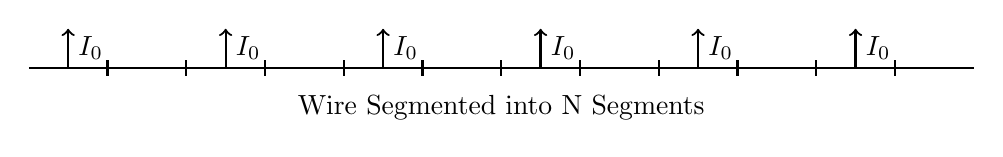
\begin{tikzpicture}
    \draw[thick] (0,0) -- (12,0);
    \foreach \x in {1,2,...,11}
        \draw[thick] (\x,0.1) -- (\x,-0.1);
    \foreach \x in {0,2,...,10}
        \draw[->, thick] (\x+0.5,0) -- (\x+0.5,0.5) node[midway,right] {$I_0$};
    \node at (6,-0.5) {Wire Segmented into N Segments};
\end{tikzpicture}
\end{center}

This diagram illustrates the wire as a series of segments, with each segment carrying a uniform current \(I_0\), thereby succinctly summarizing the principle behind the Method of Moments analysis.
